\section{Task 2}
Die Abbildungen \ref{fig::avgtime Depth2.1} und \ref{fig::avgtime Depth 2.2} zeigen die durchschnittlichen Bedenkzeiten pro Zug auf zehn verschiedenen Maps. Die Daten wurden erhoben indem jeweils ein gesamtes Spiel auf der Map gespielt wurde mit eingeschalteten Perfomance-Logging und anschließend der ausgegebene Log geparsed wurde.
%\begin{figure}[h]
%	\begin{center}
%		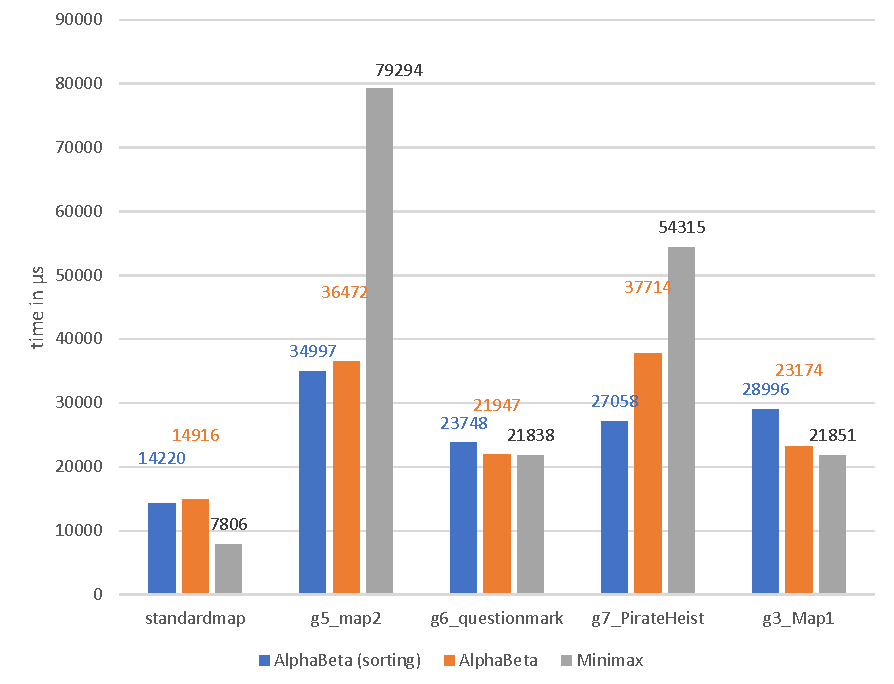
\includegraphics{Depth_1_avgtime.pdf}
%		\caption{Durchschnittszeit bei Tiefe 1}
%		\label{fig::avgtime Depth1}
%	\end{center}
%\end{figure}
\begin{figure}[h]
	\begin{center}
		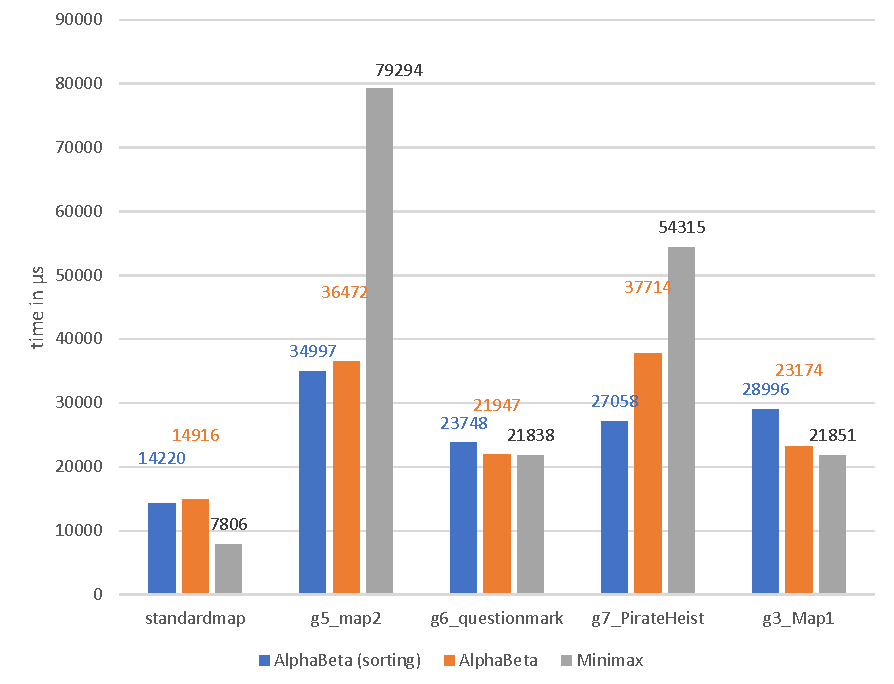
\includegraphics{Depth_2_1_avgtime.pdf}
		\caption{Durchschnittszeit bei Tiefe 2 (1/2)}
		\label{fig::avgtime Depth2.1}
	\end{center}
\end{figure}
\begin{figure}[h]
	\begin{center}
		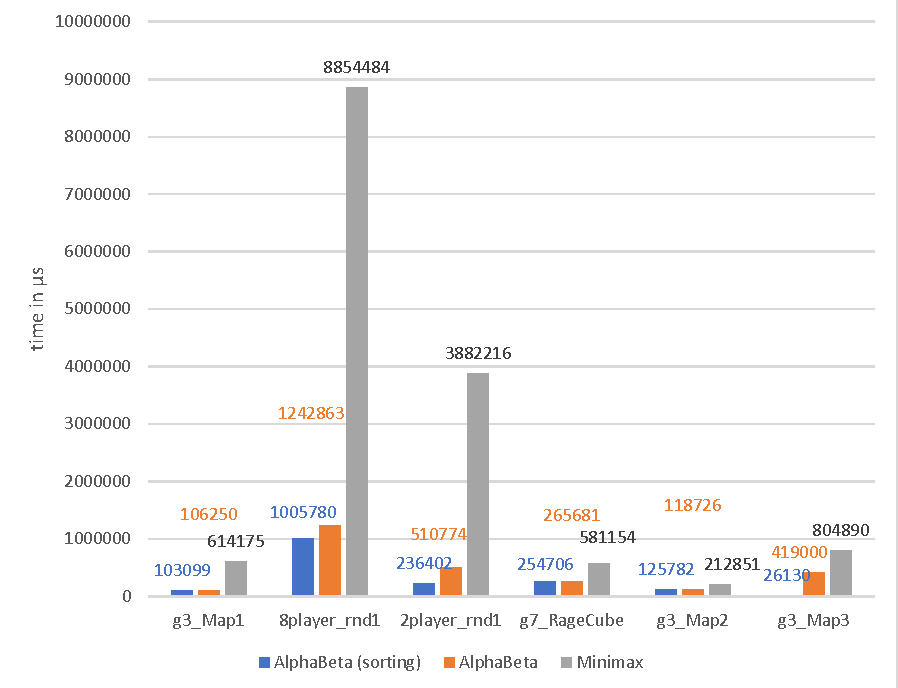
\includegraphics{Depth_2_2_avgtime.pdf}
		\caption{Durchschnittszeit bei Tiefe 2 (2/2)}
		\label{fig::avgtime Depth 2.2}
	\end{center}
\end{figure}
Es war zu erwarten, dass die durchschnittliche Bedenkzeit beim Alpha-Beta Algorithmus mit Zugsortierung stets geringer ist, als die ohne Sortierung. Leider entsprechen unsere Messungen nicht ganz den Erwartungen. So liegt in Abbildung \ref{fig::avgtime Depth2.1} häufiger die Bedenkzeit \textbf{Zugsortierung}

%\begin{figure}[h]
%	\begin{center}
%		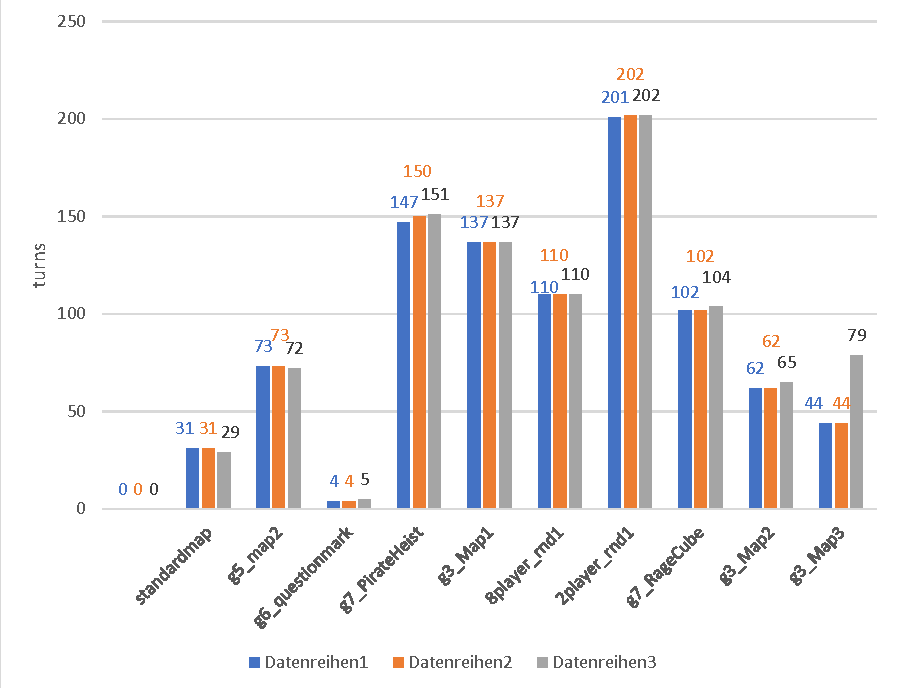
\includegraphics{Depth_1_turns.pdf}
%		\caption{Anzahl der Züge bei Tiefe 1}
%		\label{fig::turns Depth1}
%	\end{center}
%\end{figure}